%% ----------------------------------------------------------------------------
%%  §8.6  Appendice: integrabilità delle funzioni continue e monotòne
%% ----------------------------------------------------------------------------
\section{Appendice: integrabilità delle funzioni continue e monotòne}
\label{sec:integrabilita-continue}

Possiamo ora dimostrare il risultato che rende la teoria dell'integrale utilizzabile in
pratica: tutte le funzioni continue in un intervallo chiuso e limitato sono
integrabili. Lo otterremo in una forma più forte, che riguarda \emph{tutte} le
partizioni di ampiezza sufficientemente piccola, e che giustificherà le formule di
quadratura numerica.

\begin{teorema}[Integrabilità delle funzioni continue]\label{teo:integrabilita-continue}
\index{funzione!continua!integrabilità}
Sia $f$ una funzione continua in $[a,b]$. Allora $f$ è integrabile secondo Riemann in
$[a,b]$. Più precisamente, per ogni $\epsilon>0$ esiste $\delta>0$ tale che
\begin{equation}\label{eq:ampiezza-piccola}
  \abs P<\delta \ \implica\ S(P)-s(P)<\epsilon \qquad\text{per ogni partizione $P$ di }
  [a,b] .
\end{equation}
\end{teorema}

\begin{schema}
\Ipotesi{$f$ continua in $[a,b]$, $a<b$.}
\Tesi{$f$ integrabile in $[a,b]$; \ $\perogni\epsilon>0\ \esiste\delta>0$ :
$\abs P<\delta\implica S(P)-s(P)<\epsilon$.}
\end{schema}

\begin{strategia}
Per la \eqref{eq:S-s-oscillazioni} basta rendere tutte le oscillazioni $M_{k}-m_{k}$
minori di $\frac\epsilon{b-a}$: allora $S(P)-s(P)<\frac\epsilon{b-a}\sum\Delta
x_{k}=\epsilon$. Il teorema di Weierstrass assicura che $m_{k}$ e $M_{k}$ sono valori di
$f$ in due punti dell'intervallo $[x_{k-1},x_{k}]$, la cui distanza non supera
l'ampiezza della partizione; il teorema di Cantor fornisce un $\delta$, \emph{uguale per
tutti gli intervalli}, che rende piccola la differenza tra due valori di $f$ in punti
distanti meno di $\delta$.
\end{strategia}

\begin{dimostrazione}
La funzione $f$ è limitata per il teorema di Weierstrass, quindi le somme integrali
sono definite. Fissato $\epsilon>0$, per il teorema di Cantor (\cref{teo:cantor}) $f$ è
uniformemente continua in $[a,b]$, ed esiste $\delta>0$ tale che
\begin{equation}\label{eq:cantor-integrabilita}
  \abs{f(x)-f(x')}<\frac\epsilon{b-a} \qquad\text{per ogni } x,x'\in[a,b] \text{ con }
  \abs{x-x'}<\delta .
\end{equation}
Sia $P=\set{x_{0},\dots,x_{n}}$ una partizione con $\abs P<\delta$. In ogni intervallo
$[x_{k-1},x_{k}]$ la funzione continua $f$ assume minimo e massimo (\cref{teo:weierstrass}):
esistono $\xi_{k},\eta_{k}\in[x_{k-1},x_{k}]$ con $m_{k}=f(\xi_{k})$ e $M_{k}=f(\eta_{k})$.
Poiché $\abs{\xi_{k}-\eta_{k}}\le\Delta x_{k}\le\abs P<\delta$, per la
\eqref{eq:cantor-integrabilita}
\[
  M_{k}-m_{k}=f(\eta_{k})-f(\xi_{k})<\frac\epsilon{b-a} \qquad\perogni k=1,\dots,n ,
\]
e quindi
\[
  S(P)-s(P)=\sum_{k=1}^{n}(M_{k}-m_{k})\,\Delta x_{k}
  <\frac\epsilon{b-a}\sum_{k=1}^{n}\Delta x_{k}=\epsilon .
\]
Questo prova la \eqref{eq:ampiezza-piccola}. Partizioni di ampiezza minore di $\delta$
esistono (ad esempio la partizione uniforme in $n$ parti, con $n>\frac{b-a}\delta$), e il
criterio di integrabilità (\cref{teo:criterio-integrabilita}) dà l'integrabilità di
$f$.
\end{dimostrazione}

La forma forte \eqref{eq:ampiezza-piccola} ha una conseguenza importante: per una
funzione continua, l'integrale è il limite di \emph{qualsiasi} successione di somme di
Riemann, purché l'ampiezza delle partizioni tenda a zero.

\begin{teorema}[Convergenza delle somme di Riemann]\label{teo:riemann-continue}
Sia $f$ continua in $[a,b]$, sia $P_{n}$ una successione di partizioni di $[a,b]$ con
$\abs{P_{n}}\to0$, e sia $\sigma_{n}$ una somma di Riemann \eqref{eq:somma-riemann}
relativa a $P_{n}$, con punti $\xi_{k}$ scelti in modo arbitrario. Allora
\begin{equation}\label{eq:riemann-limite}
  \lim_{n\to+\infty}\sigma_{n}=\int_{a}^{b}f(x)\,dx .
\end{equation}
\end{teorema}

\begin{schema}
\Ipotesi{$f$ continua in $[a,b]$; \ $\abs{P_{n}}\to0$; \ $\sigma_{n}$ somma di Riemann
relativa a $P_{n}$.}
\Tesi{$\sigma_{n}\to\int_{a}^{b}f$.}
\end{schema}

\begin{strategia}
Ogni somma di Riemann dista dall'integrale al più $S(P)-s(P)$ \eqref{eq:riemann-stima}, e
questa quantità è piccola quando l'ampiezza della partizione è piccola, per la
\eqref{eq:ampiezza-piccola}.
\end{strategia}

\begin{dimostrazione}
Sia $\epsilon>0$ e sia $\delta$ quello del \cref{teo:integrabilita-continue}. Poiché
$\abs{P_{n}}\to0$, esiste $\nu$ tale che $\abs{P_{n}}<\delta$ per ogni $n>\nu$; per tali $n$,
la \eqref{eq:riemann-stima} e la \eqref{eq:ampiezza-piccola} danno
$\bigl|\sigma_{n}-\int_{a}^{b}f\bigr|\le S(P_{n})-s(P_{n})<\epsilon$.
\end{dimostrazione}

In particolare, per $f$ continua le medie aritmetiche di $n$ campioni equispaziati,
come quelle considerate all'inizio del \cref{sec:media}, tendono alla media integrale.

\subsection{Funzioni monotòne}

La continuità è sufficiente ma non necessaria per l'integrabilità: la funzione
dell'\cref{oss:media-discontinua} è discontinua ma integrabile. Un'altra classe
importante di funzioni integrabili, che comprende funzioni discontinue, è quella delle
funzioni monotòne.

\begin{teorema}[Integrabilità delle funzioni monotòne]\label{teo:integrabilita-monotone}
\index{funzione!monotòna!integrabilità}
Sia $f$ monotòna in $[a,b]$. Allora $f$ è integrabile secondo Riemann in $[a,b]$, e per
la partizione uniforme $P_{n}$ in $n$ parti risulta
\begin{equation}\label{eq:monotone-S-s}
  S(P_{n})-s(P_{n})=\frac{\abs{f(b)-f(a)}\,(b-a)}n .
\end{equation}
\end{teorema}

\begin{schema}
\Ipotesi{$f$ monotòna in $[a,b]$.}
\Tesi{$f$ integrabile; \ $S(P_{n})-s(P_{n})=\abs{f(b)-f(a)}\frac{b-a}n$.}
\end{schema}

\begin{strategia}
È il calcolo già fatto per $x^{2}$, per la distribuzione ellittica e per
$e^{-x^{2}}$: in ogni intervallo gli estremi di una funzione monotòna sono i valori negli
estremi dell'intervallo, e la differenza tra le somme è telescopica.
\end{strategia}

\begin{dimostrazione}
Una funzione monotòna in $[a,b]$ è limitata, perché i suoi valori sono compresi tra
$f(a)$ e $f(b)$. Sia $f$ crescente e sia $x_{k}=a+k\frac{b-a}n$. Per
$x\in[x_{k-1},x_{k}]$ si ha $f(x_{k-1})\le f(x)\le f(x_{k})$, e i valori $f(x_{k-1})$,
$f(x_{k})$ sono assunti; quindi $m_{k}=f(x_{k-1})$ e $M_{k}=f(x_{k})$, e
\[
  S(P_{n})-s(P_{n})=\frac{b-a}n\sum_{k=1}^{n}\bigl[f(x_{k})-f(x_{k-1})\bigr]
  =\frac{b-a}n\bigl[f(b)-f(a)\bigr] .
\]
Se $f$ è decrescente, si scambiano i ruoli di $x_{k-1}$ e $x_{k}$ e si ottiene
$\frac{b-a}n\bigl[f(a)-f(b)\bigr]$. In entrambi i casi vale la \eqref{eq:monotone-S-s}, che
tende a zero, e il \cref{cor:limite-somme} dà l'integrabilità.
\end{dimostrazione}

Una funzione monotòna può avere infiniti punti di discontinuità (che sono salti, per il
\cref{cor:monotone-salti}). Ad esempio, la funzione definita in $[0,1]$ da $f(0)=0$ e
$f(x)=\frac1n$ per $\frac1{n+1}<x\le\frac1n$, $n\in\N$, è crescente, ha un salto in ciascuno
dei punti $\frac1n$ con $n\ge2$, ed è integrabile per il \cref{teo:integrabilita-monotone}.

\subsection{Formule di quadratura}

Il \cref{teo:riemann-continue} giustifica il calcolo numerico degli integrali delle
funzioni continue mediante somme di Riemann. Con la partizione uniforme di passo
$h=\frac{b-a}n$ e nodi $x_{k}=a+kh$, le formule più semplici sono quella dei
\emph{rettangoli} (con l'estremo sinistro), quella del \emph{punto medio} e quella dei
\emph{trapezi}:
\begin{align}
  R_{n}&=h\sum_{k=0}^{n-1}f(x_{k}),
  \label{eq:quadratura-rettangoli}\\
  M_{n}&=h\sum_{k=1}^{n}f\Bigl(\frac{x_{k-1}+x_{k}}2\Bigr),
  \label{eq:quadratura-medio}\\
  T_{n}&=h\Bigl[\frac{f(x_{0})+f(x_{n})}2+\sum_{k=1}^{n-1}f(x_{k})\Bigr].
  \label{eq:quadratura-trapezi}
\end{align}
Le prime due sono somme di Riemann, e convergono all'integrale per il
\cref{teo:riemann-continue}. La terza è la media aritmetica della somma dei rettangoli
con l'estremo sinistro e di quella con l'estremo destro, e converge per lo stesso
motivo; il nome deriva dal fatto che, per $f\ge0$, $T_{n}$ è la somma delle aree dei
trapezi di altezza $h$ e basi $f(x_{k-1})$, $f(x_{k})$ (\cref{fig:quadratura}).

Le tre formule non convergono però con la stessa rapidità. Per una funzione monotòna
l'errore della formula dei rettangoli non supera la \eqref{eq:monotone-S-s}, che è
dell'ordine di $\frac1n$, e in generale non è più piccolo. Per il punto medio e per i
trapezi, invece, si dimostra con la formula di Taylor (lo si fa nei corsi di Calcolo
numerico) che, se $f$ ha derivata seconda continua,
\begin{equation}\label{eq:errori-quadratura}
\begin{aligned}
  \Bigl|M_{n}-\int_{a}^{b}f\Bigr|&\le\frac{(b-a)\,h^{2}}{24}\max_{[a,b]}\abs{f''},\\
  \Bigl|T_{n}-\int_{a}^{b}f\Bigr|&\le\frac{(b-a)\,h^{2}}{12}\max_{[a,b]}\abs{f''} :
\end{aligned}
\end{equation}
raddoppiando $n$ l'errore si riduce di circa quattro volte. Inoltre l'errore del punto
medio è circa la metà di quello dei trapezi e di segno opposto, per cui la combinazione
$\frac{2M_{n}+T_{n}}3$, che è la \emph{formula di Cavalieri--Simpson}, elimina il termine
principale dell'errore. Il programma seguente lo verifica sull'integrale
$\int_{0}^{1}e^{-x^{2}}dx$ dell'\cref{es:stima-gaussiana}.

\begin{python}[Formule di quadratura a confronto]
import math

f = lambda x: math.exp(-x * x)
I = math.erf(1) * math.sqrt(math.pi) / 2     # valore di riferimento

def quadrature(f, a, b, n):
    """Rettangoli, punto medio, trapezi, Cavalieri-Simpson."""
    h = (b - a) / n
    x = [a + k * h for k in range(n + 1)]
    ret = h * sum(f(x[k]) for k in range(n))
    med = h * sum(f(x[k] + h / 2) for k in range(n))
    tra = h * (sum(f(t) for t in x) - (f(a) + f(b)) / 2)
    return ret, med, tra, (2 * med + tra) / 3

print("errori assoluti")
print(f"{'n':>4} {'rettangoli':>11} {'p. medio':>10}"
      f" {'trapezi':>10} {'Simpson':>10}")
for n in (4, 8, 16, 32, 64):
    err = [abs(q - I) for q in quadrature(f, 0, 1, n)]
    print(f"{n:4d} " + " ".join(f"{e:10.2e}" for e in err))
\end{python}
\begin{risultato}
errori assoluti
   n  rettangoli   p. medio    trapezi    Simpson
   4   7.52e-02   1.92e-03   3.84e-03   1.99e-06
   8   3.85e-02   4.79e-04   9.59e-04   1.25e-07
  16   1.95e-02   1.20e-04   2.40e-04   7.79e-09
  32   9.82e-03   2.99e-05   5.99e-05   4.87e-10
  64   4.92e-03   7.48e-06   1.50e-05   3.05e-11
\end{risultato}

\begin{figure}[htb]
\centering
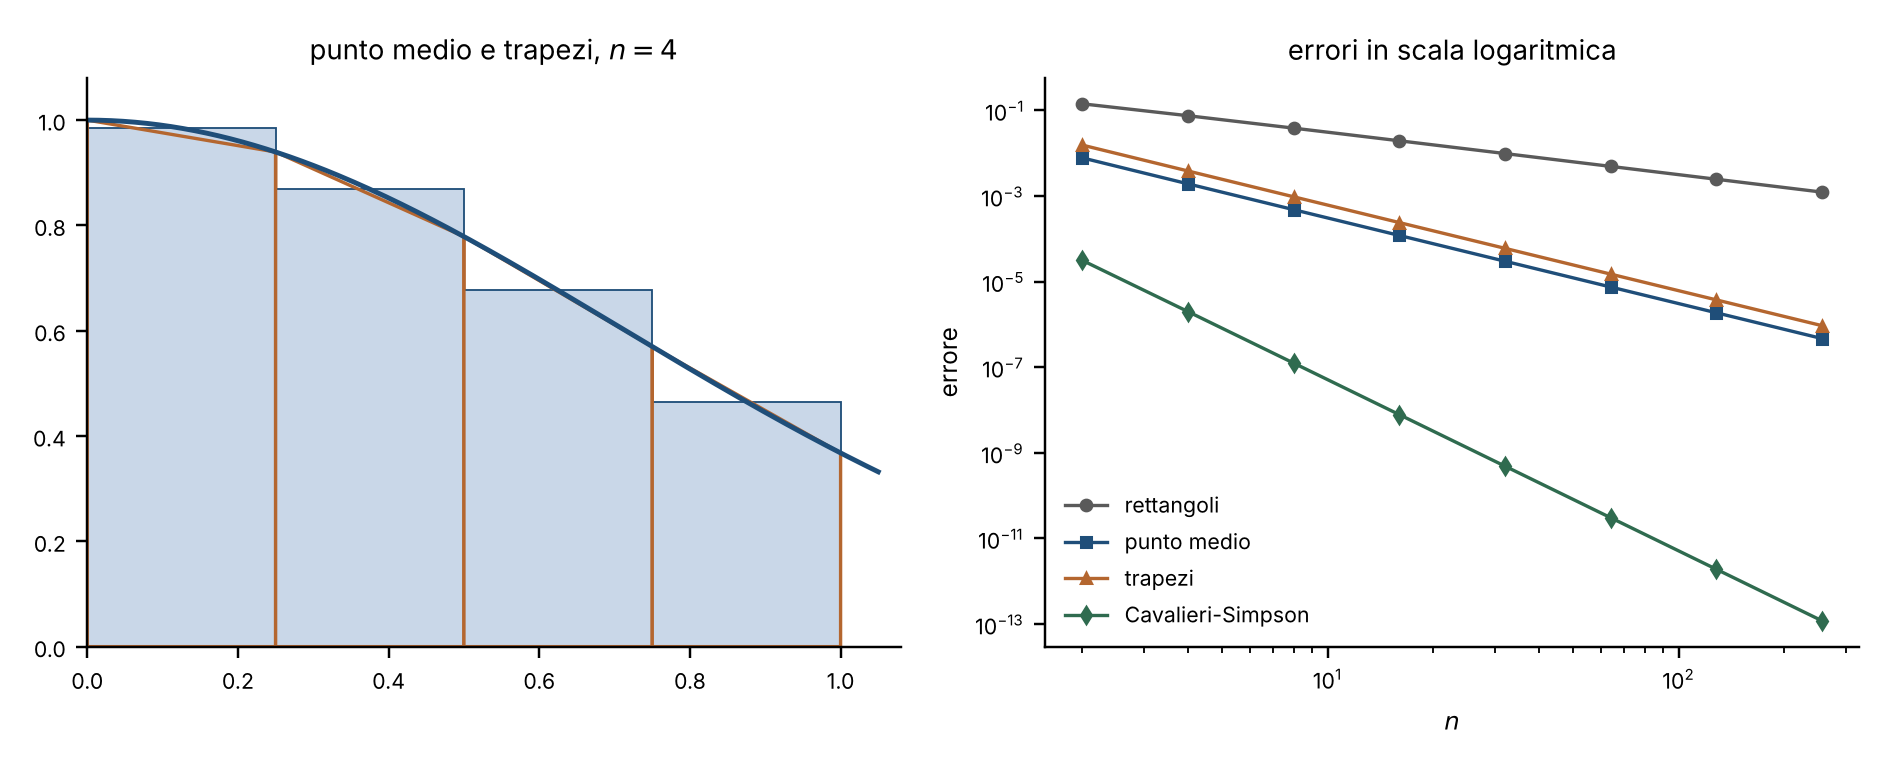
\includegraphics[width=\textwidth]{figure/quadratura.png}
\caption{A sinistra, le formule del punto medio (rettangoli azzurri) e dei trapezi
(contorni in color rame) per $e^{-x^{2}}$ in $[0,1]$ con $n=4$. A destra, gli errori
delle quattro formule in funzione di $n$, in scala logaritmica: le pendenze $-1$, $-2$
e $-4$ corrispondono a errori proporzionali a $\frac1n$, $\frac1{n^{2}}$, $\frac1{n^{4}}$
(\texttt{python/fig\_quadratura.py}).}
\label{fig:quadratura}
\end{figure}

\begin{notastorica}[Da Cauchy a Lebesgue]
Cauchy dimostrò nel 1823 che le somme costruite sugli estremi sinistri di una funzione
continua convergono, quando l'ampiezza della partizione tende a zero, a un limite
indipendente dalle partizioni: è un caso particolare del nostro
\cref{teo:riemann-continue} (sulla lacuna della dimostrazione si veda la nota del
\S\ref{sec:uniforme-continuita}). Riemann, con il suo criterio, estese l'integrale a
funzioni con infinite discontinuità: quali funzioni limitate sono integrabili?
Dirichlet, nella memoria del 1829 in cui compare la sua funzione (\cref{oss:dirichlet}),
aveva indicato come necessario che tra due punti qualsiasi si trovasse sempre un
intervallo di continuità; ma Riemann costruì una funzione integrabile discontinua in un
insieme denso. Hermann Hankel (1870) credette che un insieme non denso in alcun
intervallo si potesse racchiudere in un numero finito di intervalli di lunghezza totale
piccola a piacere; Henry Smith (1875) mostrò che non è così. La risposta
definitiva venne all'inizio del Novecento da Henri Lebesgue e, indipendentemente, da
Giuseppe Vitali (1903): sono integrabili le funzioni limitate il cui insieme dei punti di
discontinuità ha \emph{misura nulla}, cioè si può ricoprire con una successione di
intervalli di lunghezza totale piccola a piacere (come l'insieme numerabile dei salti di
una funzione monotòna, ma non $[0,1]$, dove è discontinua la funzione di Dirichlet).
Quanto alle formule di quadratura, quella che in Italia porta il nome di
Cavalieri--Simpson era nota, in forme equivalenti, a Keplero, che nel 1615 la usò per
stimare il volume delle botti, a Bonaventura Cavalieri e a James Gregory, prima che
Thomas Simpson la diffondesse nel 1743.
\end{notastorica}
